\documentclass{standalone}
\usepackage{pgfplots}
\pgfplotsset{compat=1.18}
\usetikzlibrary{decorations.pathreplacing}

\begin{document}
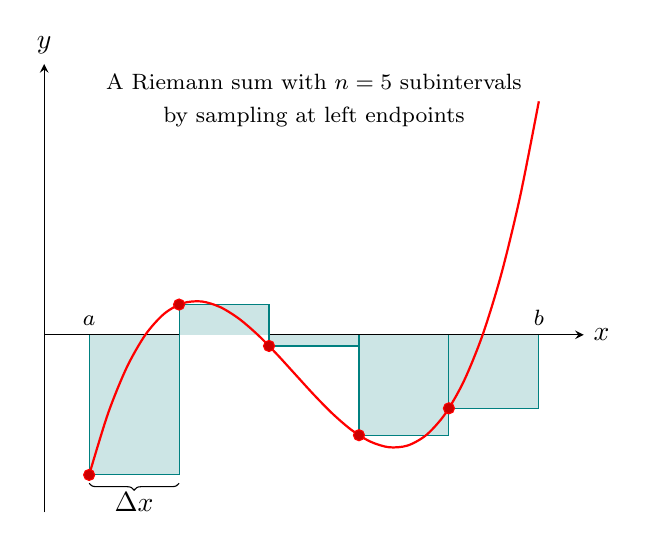
\begin{tikzpicture}
  \begin{axis}[
    axis lines=center,
    xlabel={\(x\)},
    ylabel={\(y\)},
    xlabel style={at={(ticklabel* cs:1)}, anchor=west},
    ylabel style={at={(ticklabel* cs:1)}, anchor=south},
    enlargelimits=true,
    axis line style={thin},
    xtick=\empty,
    ytick=\empty,
    black,
    ]

    \addplot +[draw=teal,fill=teal!20,no markers] coordinates { (0.500,0) (0.500,-2.625) (1.300,-2.625) (1.300,0) };
    \addplot +[draw=teal,fill=teal!20,no markers] coordinates { (1.300,0) (1.300,0.567) (2.100,0.567) (2.100,0) };
    \addplot +[draw=teal,fill=teal!20,no markers] coordinates { (2.100,0) (2.100,-0.209) (2.900,-0.209) (2.900,0) };
    \addplot +[draw=teal,fill=teal!20,no markers] coordinates { (2.900,0) (2.900,-1.881) (3.700,-1.881) (3.700,0) };
    \addplot +[draw=teal,fill=teal!20,no markers] coordinates { (3.700,0) (3.700,-1.377) (4.500,-1.377) (4.500,0) };

    \addplot +[mark=*, only marks] coordinates { (0.500,-2.625) (1.300,0.567) (2.100,-0.209) (2.900,-1.881) (3.700,-1.377) };

    \addplot[thick, red, domain=0.5:4.5, smooth] {(x-1)*(x-2)*(x-4)};

    % % Braces and labels without any loops
    \draw[decorate, decoration={brace, mirror, raise=3pt}]
      (axis cs:0.5,-2.625) -- (axis cs:1.3,-2.625)
      node[midway,below=3pt] {\(\Delta x\)};

  \node[below,align=center] at (current axis.north) {\footnotesize A Riemann sum with \(n=5\) subintervals\\\footnotesize by sampling at left endpoints};

    \node[above] at (axis cs:0.5,0) {\footnotesize \(a\)};
    \node[above] at (axis cs:4.5,0) {\footnotesize \(b\)};
  \end{axis}
\end{tikzpicture}
\end{document}
